\section{Memory}

Applications written for Grappa utilize two forms of memory: local and global.
Local memory is local to a single core \comment{core or processor/node?} in
the system. Accesses occur through conventional pointers. The compiler emits
an access and the memory is manipulated directly. Applications use local
accesses for a number of things in Grappa: the stack associated with a task,
accesses to localized global memory in caches (see below), and accesses to
debugging infrastructure that is local to each system node. Local pointers
cannot access memory on other cores, and are valid only on their home core.

Large data that is expected to be shared and accessed with low locality is
stored in Grappa's global memory. All global data must be accessed through
calls into Grappa's API, shown in Figure~\ref{fig:accessing-memory}.

\paragraph{Global memory addressing} Grappa provides two methods for storing
data in the global memory. The first is a distributed heap striped across all
the machines in the system in a block cyclic fashion. The
\texttt{global\_malloc} and \texttt{global\_free} calls are used to allocate
and deallocate memory in the global heap. Addresses to memory in the global
heap use \textbf{linear addresses}. Choosing the block size involves trading
off sequential bandwidth against aggregate random access bandwidth. Smaller
block sizes help spread data across all the memory controllers in the cluster,
but larger block sizes allow the locality-optimized memory controllers to
provide increased sequential bandwidth. The block size, which is configurable,
is typically set to 64 bytes, or the size of a single hardware cache line, in
order to exploit spatial locality when available. 

%%% is the below important? -Luis
\comment{The heap metadata is stored on a single node. Currently all heap
allocation and free operations are serialized through this node; while this
has been sufficient for our benchmarks, it is easy to relax in the future
Grappa will provide parallel performance through
combining~\cite{MAMA,flatcombining}.}

Grappa also allows any local data on a core's stacks or heap to be
exported to the global address space to be made accessible to other
cores across the system. Addresses to global memory allocated in this
way use \textbf{2D global addresses}.  This uses a traditional PGAS
addressing model, where each address is a tuple of a rank in the job (or
global process ID) and an address in that process. The lower 48 bits of
the address hold a virtual address in the process. The top bit is set to
indicates that the reference is a 2D address (as opposed to linear
address). This leaves 15 bits for network endpoint ID, which limits our
scalability to $2^{15}$ endpoints. Any node-local data can be made
accessible by other nodes in the system by wrapping the address and node
ID into a 2D global address. This address can then be accessed with a
delegate operation and even be cached by other nodes. The
address is converted at the destination into a canonical x86 address by replacing the upper
bits with the sign-extended upper bit of the virtual address. 2D
addresses may refer to memory allocated from a single processes' heap or
from a task's stack. Figure~\ref{fig:memory-structure} shows how 2D and
linear addresses can refer to other cores' memory.


\begin{figure}[htbp]
  \begin{center}
    \begin{minipage}{\columnwidth}
	\small
	\begin{tabular}{l}
      	\texttt{\scriptsize global\_address global\_malloc( size )} \\
      	\texttt{\scriptsize global\_free( global\_address )} \\ 
      	Allocation in the global heap \\ \\
      	\texttt{\scriptsize delegate\_read( global\_address, local\_var )}  \\
      	\texttt{\scriptsize delegate\_write( global\_address, local\_var )} \\
      	\texttt{\scriptsize delegate\_cas( global\_address, local\_var )} \\
      	\texttt{\scriptsize delegate\_fetch\_inc( global\_address, local\_var )} \\ 
      	Memory operations at the home core of a global address \\ \\
      	\texttt{\scriptsize cache\_acquire( global\_address, local\_buf, \{RO,RW,WO\})} \\
      	\texttt{\scriptsize cache\_release( global\_address, local\_buf )} \\ 
		Perform cache operations to acquire/release global data.  \\
		Acquire copies all data to local node and returns a pointer. \\ 	
		Release optionally copies data back to global memory. \\
	\end{tabular}
      \caption{\label{fig:accessing-memory} Grappa API for memory accesses}     \end{minipage}
  \end{center}
\end{figure}

\begin{figure}[t]
\begin{center}
  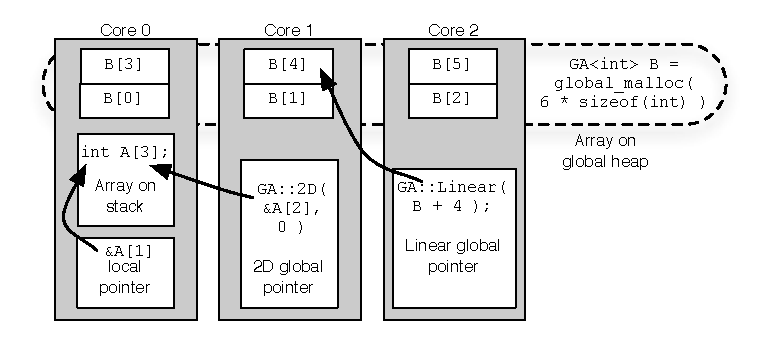
\includegraphics[width=0.95\columnwidth]{figs/memory-structure}
\begin{minipage}{0.95\columnwidth}
  \caption{\label{fig:memory-structure} Global memory referencing in Grappa}
\end{minipage}
\vspace{-3ex}
\end{center}
\end{figure}

\paragraph{Global memory access} There are two general approaches
Grappa applications use to {\emph access} global memory. When the
programmer expects a computation on shared data to have spatial locality
to exploit, {\em cache} operations may be used. When there is no
locality to exploit, {\em delegate} operations are used.

\textit{Explicit caching.} Grappa provides an API to fetch a global pointer of
any length and return a local pointer to a cached copy of the global memory.
Grappa cache operations have the usual read-only and read-write variants,
along with a write-only variant used to initialize data structures. Languages
for distributed shared memory systems have done optimizations to achieve a
similar goal. For example, the UPC compiler coalesces struct and array
accesses into remote get/put \cite{Chen:2005}, and Fortran D compiler's
message vectorization hoists small messages out of a loop
\cite{FortranD:1992}. Caching in Grappa additionally provides a mechanism for
exploiting temporal locality when available by operating on the data locally.

Under the hood, Grappa performs the mechanics of gathering chunks of data from
multiple system nodes and presenting a conventional appearing linear block of
memory as a local pointer into a cache. The strategy employed is to issue all
the constituent requests of the desired block (as Active Messages) and then
yield until all responses have occurred. Currently, Grappa caches are
\emph{not} kept coherent automatically. If that is desired, the programmer to
is responsible for pushing the updated block back to its home node. Given that
synchronization is explicit in Grappa, we don't expect this to be a
significant burden (programmers can push updates before a relevant
synchronization operation).

% Future work will develop a software directory based coherence scheme to
% simplify consistent access to global data.

\textit{Delegate operations.} When the access pattern has low-locality,
it is more efficient to modify the data on its home core rather than
bringing a copy to the requesting core and returning it after
modification. Delegate operations provide this capability. Applications
can dispatch computation to be performed on individual machine-word
sized chunks of global memory to the memory system itself (e.g.,
\emph{fetch-and-add}).  Delegate operations, proposed in
\cite{Nelson:hotpar11} and \cite{delegated:oopsla11}, are also the
primary synchronization method in Grappa.

Delegate operations are always executed at the home core of their
address, and while arbitrary memory operations can be delegated, we
restrict the use of delegate operations in three ways to make them more
useful for synchronization. First, we limit each task to one outstanding
delegate operation to avoid the possibility of reordering in the
network. Second, we limit delegate operations to operate on objects in
the 2D address space or objects that fit in a single block of the linear
address space so they can be satisfied with a single network request.
Finally, no context switches are allowed while the data is being
modified. Given these restrictions, we can ensure that delegate
operations for the same address from multiple requesters are always
serialized through a single core in the system, providing atomic
semantics without using actual atomic operations (and thus avoiding their typical high cost). 
Figure~\ref{fig:delegate-cache} depicts an example of how delegate and
cache operations interact.

\begin{figure*}[htb] \begin{center}
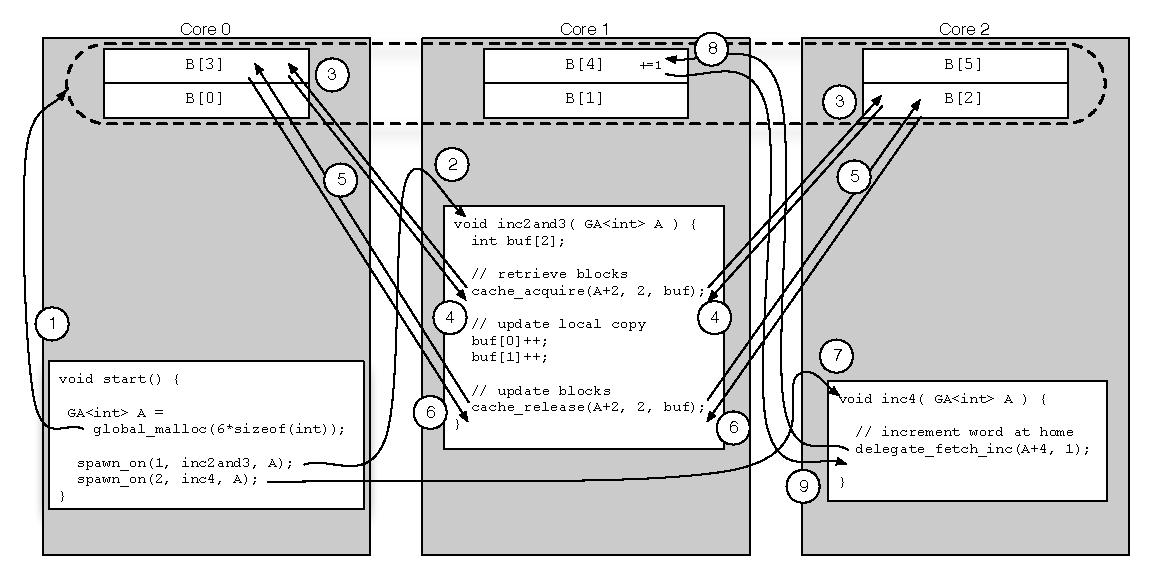
\includegraphics[width=1.5\columnwidth]{figs/delegate-cache}
\begin{minipage}{1.9\columnwidth} \caption{\label{fig:delegate-cache}
\textbf{Delegation and cache example:} A core allocates an array in the global
heap (1). It then spawns two tasks on remote cores to increment elements of
the array. The first task increments two elements of the array using cache
operations. The first task is then invoked (2). A cache request is issued for two
adjacent integers starting at the second element of the array. Since these
element are stored in the memories of two different cores, this requires two messages to be sent (3). The task is suspended until both responses arrive
(4). The data carried in these responses is stored in the local buffer. The
elements are then incremented in the buffer. The modified data is then sent back
to the home node (5). Acknowledgements are returned (6) so the task
knows when the writes are complete. The second task increments an element of
the array with a delegate operation. The task is invoked (7). A delegate
request is sent to the home core of the array element with the increment
value. The task suspends until the response is received. The increment
is executed on the remote core (8). A response is returned (9) with the
previous value of the array element. } \end{minipage} \vspace{-3ex}
\end{center} \end{figure*}

\paragraph{Memory consistency model discussion} As mentioned earlier, all
synchronization operations are done via delegate operations. Since they all
execute in their home node, they are guaranteed to be serialized , with their
updates visible to all cores across the system in the same order. Also, tasks
are restricted to a single outstanding delegate operation at a time, and
therefore are not subject to potential request reordering. Consequently, all
synchronization operations execute in program order and are made visible in
the same order to all cores in the system. These properties are sufficient to
guarantee a memory model that offers sequential consistency for data-race-free
programs~\cite{drf} (all accesses to shared data are separated by
synchronization). This is the memory model that underpins C/C++.

Note, however, that if the application code uses explicit caching on shared
data, all updates must be sent back to the home node before the
synchronization operation that protects the data is performed. 



